\chapter{Design and Methodology}
Chapter Three provides a detailed description of the design decisions for the research, building on the foundations and stemming from the related work reviewed in Chapter Two. Firstly, the data is gathered to ensure that the research objectives and challenges outlined in Chapter One are met. In the second phase, the neural translation model is designed to generate translation in the target language and finally a visual interface is designed to display the translations.

\begin{figure}[h]
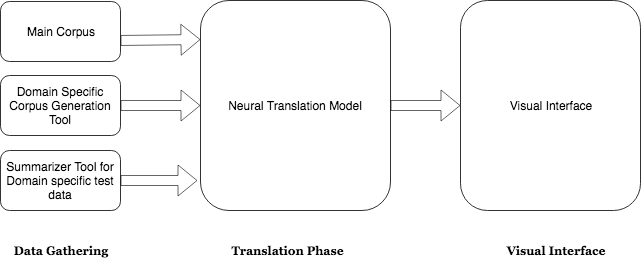
\includegraphics[width=\textwidth]{figures/maindesign.png}
\caption{Phases of the Design process} \label{maindesign}
\end{figure}

\section{Data Gathering}
The first phase of Data Gathering relate to the process of corpus selection, detailed by the research objective:Select a large Hindi-English Corpus to train the neural translation model.
\subsection{IIT Bombay English-Hindi Parallel Corpus}
IIT Bombay English-Hindi Parallel Corpus was presented by \cite{Kunchukuttan2018TheIB}. The corpus is a compilation of parallel corpora which was previously available in the public domain as well as the new corpus they collected.Currently there is unavailability of large parallel corpus in Hindi-English containing multi-domain data, which is very necessary for neural machine translation.The decision to use IIT-Bombay English-Hindi Parallel Corpus was due its large size and quality of data it contains. It is the largest publicly available English-Hindi parallel corpus and was presented in 11th edition of the Language Resources and Evaluation Conference 2018. The corpus contains 1.49 million parallel sentence segments of which 694K segments are newly collected and not previously available in the public domain, which makes it perfect fit for this neural machine translation task. 

The parallel corpus has been compiled form a variety of existing sources like OPUS (\cite{TIEDEMANN12.463}), HindEn (\cite{11858/00-097C-0000-0023-625F-0}) and TED (\cite{Abdelali2014TheAC})) as well as the corpora developed at the Centre for Indian Language Technology, IIT Bombay over the years. The training corpus is consisted of sentences, phrases , dictionary entries spanning across multiple applications and domains. The details of the training set have been shown in Table 3.1.

\subsubsection{Corpus Details}
The details of the new sub-corpora that was added to the collection for the IIT Bombay English-Hindi Parallel Corpus are as follows.

\textbf{Judicial domain corpus - I} contains translations of legal judgments by in-house translators with many years with many years of translation experience though they didn’t have knowledge of the legal domain.

\textbf{Judicial domain corpus - II} contains translation done by graduate student who took part in a graduate course on natural language processing. This exercise was part of collecting translation in a complex domain by non-expert translators. The translations included in the corpus were determined to be of good quality by annotators.

\textbf{Mahashabdkosh 2} is an online official terminology dictionary website which is hosted by Department of Official Language, India. It contains Hindi and its equivalent English definitions. The translation sentence pairs were crawled from the official website.

\textbf{Indian Government corpora} was manually collected by the staff form Center for Indian Language Technology from various government websites like the National Portal of India, Reserve Bank of India, Ministry of Human Resource Development, NABARD,etc.

\textbf{Hindi-English Linked Wordnet} contains bilingual dictionary entries created from the linked Hindi and English wordnets.

\textbf{Gyaan-Nidhi Corpus} is a million pages multilingual parallel text corpus in English and 11 Indian languages (Assamese, Bengali, Gujarati, Hindi, Kannada, Marathi, Malayalam, Oriya, Punjabi, Tamil \& Telugu) based on Unicode encoding. The authors performed sentence alignment technique proposed by Moore (2002) to extract the parallel corpora from this comparable corpora. 

\begin{table}[h]
\centering
\resizebox{\textwidth}{!}{\begin{tabular}{rrr}
  \hline \textbf{Corpus Id} & \textbf{Source} & \textbf{Number of Segments} \\ 
  \hline
  1&GNOME (OPUS) (Tiedemann, 2012))&145,706\\
  2&KDE4 (OPUS) &97,227\\
  3&Tanzil (OPUS)&187,080\\
  4&Tatoeba (OPUS)&4,698\\
  5& OpenSubs2013 (OPUS)&4,222\\
  6& HindEnCorp (Bojar et al., 2014b)&273,885\\
  7&Hindi-English Linked Wordnets (Bhattacharyya, 2010)& 175,175\\
  8&Mahashabdkosh: Administrative Domain Dictionary
(Kunchukuttan et al., 2013)&66,474\\
9&Mahashabdkosh: Administrative Domain Examples &46,825\\
10& Mahashabdkosh: Administrative Domain Definitions&46,523\\
11&TED talks (Abdelali et al., 2014) &42,583\\
12&Indic Multi-parallel corpus (Alexandra Birch and Post, 2011)&10,349\\
13&Judicial domain corpus - I (Kunchukuttan et al., 2013)&5,007\\
14&Judicial domain corpus - II (Kunchukuttan et al., 2012)&3,727\\
15&Indian Government corpora&123,360\\
16&Wiki Headlines (Provided by CMU: www.statmt.org/wmt14/wiki-titles.tgz)&32,863\\
17& Gyaan-Nidhi Corpus &227,123\\
\hline
\textbf{Total}&&\textbf{1,492,827}\\
\hline
\end{tabular}}
\caption{Details of the IITB English-Hindi Parallel Corpus (training set)}
\end{table}

\subsubsection{Corpus Statistics}
The test and dev corpora used in the IIT Bombay Hindi-English Corpus are the same ones that was used for the WMT 2014 English-Hindi shared task (Bojar et al., 2014a) which contains newswire sentences. The detailed statistics about the whole dataset is shown in Table 3.3.

\begin{table}[h!]
\centering
 \begin{tabular}{ |ccc| } 
  \hline \textbf{Set} & \textbf{Description} & \textbf{Number of Segments}  \\ 
  \hline
  Dev (use for tuning)& Newswire (from WMT 2014)&520\\
  Test (use for final evaluation)& Newswire (from WMT 2014) &2507\\
  \hline
 \end{tabular}
\caption{Details of the IITB English-Hindi Parallel Corpus (Dev and Test set)}
\end{table}

\begin{table}[h!]
\centering
 \begin{tabular}{ |ccccc| } 
  \hline &\textbf{Language} & \textbf{Train} & \textbf{Test} & \textbf{Dev} \\ 
  \hline 
  \#Sentences && 1,492,827&2,507& 520\\
  \hline
  \#Tokens& eng&20,667,259 &57,803& 10,656\\
  &hin& 22,171,543&63,853&10,174\\
  \hline
  \#Types&eng&250,782&8,957& 2,569\\
  &hin& 343,601&8,489& 2,625\\
  \hline
 \end{tabular}
\caption{Statistics of data sets}
\end{table}

\subsubsection{Corpus Quality}
The IIT Bombay Hindi-English Parallel Corpus contains about 1.49 million Hindi – English sentence pairs which is an excellent fit for Neural Machine Translation. Though the Neural Machine Translation models demand much larger parallel corpora for better performance, but this corpus  is sufficient to train an efficient model. This corpus achieved the benchmark on baseline SMT and NMT systems and was also used for the three shared tasks (Workshop on Asian Language Translation 2016, 2017 and 2018). The quality of corpus also depends on its content, the data in this corpus is collected from multiple domains which makes it fitter for neural machine translation. The corpus contains data from domains such as Judicial , Health , Tourism , Administrative etc making it more apt for creating a generic neural translation model which works efficiently irrespective of domain.
All the data (training, dev and text) in the parallel corpus is normalized and tokenized which makes it easier for training neural translation models. For Hindi, the Indic NLP library(\cite{Kunchukuttan2013}) was used , whereas for English the Moses tokenizer was used.  

\subsubsection{Monolingual Corpus}
\label{sec:mono}
IIT-Bombay Hindi-English Parallel Corpus also provides a Hindi Monolingual Corpus which contains about 45 million sentences. This monolingual data contains data from various multi domain sources such as BBC, Health Domain, Toursim Domain, Wikipedia and Judicial domain. As discussed in the State of Art , use of monolingual data in Neural Machine Translation has shown improvements in translation quality. The monolingual corpus can be used to improve the translation quality by using the Back Translation method as suggested by \cite{DBLP:journals/corr/SennrichHB15a}.

\subsection{Domain specific Corpus Generation for Fine Tuning}
The second phase of Data Gathering relate to the process of corpus generation, detailed by the research objective: Gather a corpus of TED talks transcript in Hindi and English to fine- tune the system. The word \textit{fine-tune} refers to the process of re-training a pre-trained model with domain-specific corpus.

\subsubsection{TED Talks} 
TED Talks are a series of influential videos from expert speakers on various topics such as education, science, politics, creativity with availability in more than 100 languages. TED concurrently runs the TED Translator program where the existing TED talks are translated to different languages either through speech translation or through transcripts. The decision to use TED Talks transcripts to create a corpus for fine tuning was motivated by few factors. TED has around 411 videos for which transcripts are available in Hindi and English which is sufficient to create a corpus for fine tuning the trained neural translation model. Secondly, the data in TED talks are experiences of the speakers which is quite similar to the travel blogs, experiences of the travellers. 

\subsubsection{Parallel Corpus Generation}

The system must be capable of generating a corpus which represents the sentences pairs in Hindi and English. 

Corpus Generation is an extensive field of research on its own. It is important for this work, that a method for corpus generation is intuitively decided upon, to allow for the subsequent neural translation model training that is the core interest and aim of this research.The corpus generation process of the IIT Bombay Hindi-English Corpus (\cite{Kunchukuttan2018TheIB}) was discussed earlier. A similar approach is considered here.

\begin{itemize}
    \item First, Using web scrapping methods to obtain the transcript from the TED talks website
    \item Second, Processing the obtained data to make it ready to be used as a parallel corpus.
\end{itemize}

The first process involves using open-source web scrapper to obtain the transcripts in Hindi and English respectively from the TED talks official website. However there is an issue with this as there is no Public API available for TED talks transcripts, a significant amount of Web research is needed to pull out the data from the website.

The second process involves processing of the data obtained in the first step. As the other works like \cite{Kunchukuttan2018TheIB} suggests the use normalization, tokenization and sentence-alignment on the corpus data, the same must be implemented in this corpus data to make it more robust.

\subsubsection{Corpus size and quality}

The system approach to corpus generation must be scalable and the corpus generated by the system must be of good quality.

The corpus must be large enough to improve the translation quality by fine-tuning the trained models. Duplication of the data must be avoided in the corpus as it may have a negative impact on the translation quality.

\subsubsection{Design Structure}

Guided by the data gathering process, software that will create the fine tuning corpus for the neural machine translation can now be designed. The requirements discussed in the previous section form the building blocks for the system design, each sub-component representing a specific functionality that must be provided by the system.The system structure is as follows:

\begin{itemize}
    \item \textbf{Web Scrapping} : The web scraping consists of retrieving the transcript texts from the TED Website in Hindi and English.
    \item \textbf{Natural Language Processing} : The natural language processing consists of processing the retrieved text in the above step using different NLP tools.
\end{itemize}

\begin{figure}[!h]
\fbox{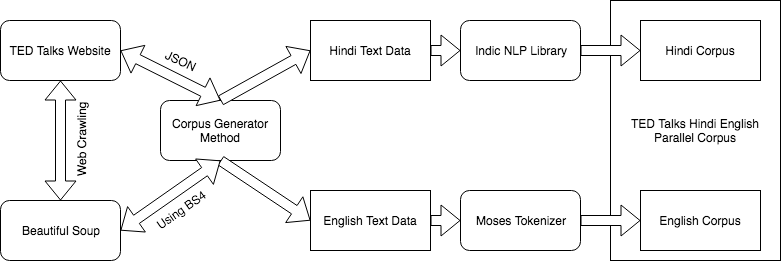
\includegraphics[width=\textwidth]{figures/design1.png}}
\caption{Components of the Corpus Generation} \label{design1}
\end{figure}

\textbf{Web-Scrapping and Text Generation}
The design structure for the processes of Web-scraping and text generation consists of the subset of components, pictured in Figure \ref{design2}.

\begin{figure}[h]
\includegraphics[width=\textwidth]{figures/design2.png}
\caption{Web scrapping components} \label{design2}
\end{figure}

\begin{itemize}
    \item \textbf{TED Talks Website} The TED Talks website contains Hindi talks which is used for the Text generation.
    \item \textbf{BeautifulSoup} It is an open-source python based library which acts as an interface between the tool and the TED Talks website.
    \item \textbf{Corpus Generator Method} This is the software which generates the corpus. First, it uses the Beautiful Soup to collect the list of talks in Hindi and ensures that there is no duplication in the list. Further it uses JSON parser to collect the texts from the transcripts which is hosted on the TED server.
\end{itemize}

The Web-scraping and text collection process involves key design decisions with regard to corpus generation. This component must be capable of retrieving the transcript texts from the TED talks website. 

The components must adhere to the requirements of \textit{ corpus size} and \textit{corpus quality}. Firstly, the tool must be scalable and be able to handle large sets of data. The tool must be robust and it should be more generic, it should have the ability to retrieve texts for any language. Secondly, the tool must avoid duplication of data, none of the TED Talks must be repeated for retrieval of data.

\begin{figure}[h]
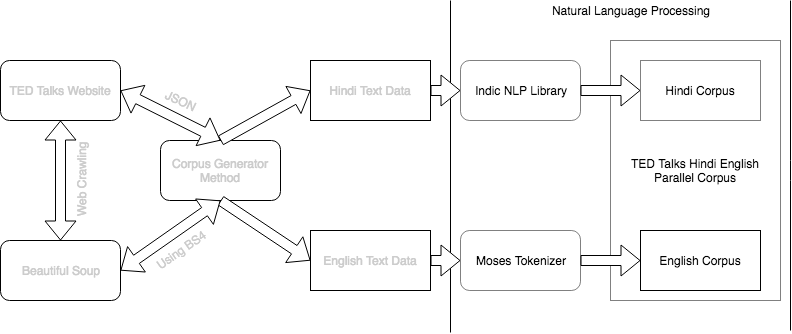
\includegraphics[width=\textwidth]{figures/design3.png}
\caption{Natural Language Processing components} \label{design3}
\end{figure}

\textbf{Natural Language Processing } The design structure for the processes of Natural Language Processing consists of the subset of components, pictured in Figure \ref{design3}.

\begin{itemize}
    \item \textbf{Text Data} The retrieved data from the first component is saved Hindi and English Text files which serves as the basic component of the Natural Language Processing component.
    \item \textbf{Indic NLP Library } It is an open-source python based library which acts as an interface between the Hindi raw text data and the processed Hindi text data. This library performs several text processing methods like normalization, tokenization and morphological analysis.
    \item\textbf{Moses Tokenier} Its an open source perl based library which is used process the English raw text data and perform normalization and tokenization.
    \item\textbf{Corpus} The final sub-component of the system is the Corpus which is the sentence aligned parallel corpus of both Hindi and English data.
\end{itemize}

Core decisions that must be made here involve the methods by which natural language processing must be done. The text must be normalized and tokenized for further use in the corpus.This component must ensure that the \textit{corpus quality} is met, the data must not be duplicated and the data must be presented in a machine readable form.

\subsection{Domain specific Test Data}
The third phase of Data Gathering relate to the process of test data generation, detailed by the research objective: Gather a list of Tripoto Blogs and create summaries for use as the domain specific test data.
\subsubsection{Tripoto}
"\textit{Tripoto is a social travel platform to share and discover  travel experiences, stories, community, tourism guides, hotels, holidays, getaways, attractions and maps}".  Tripoto contains thousands of blogs from thousands of different users on different travel related topics, it is one of the biggest open access blog websites which lets its user to share their content. The blogs contains travel experiences, itineraries, photo stories and travel related articles about different places from different parts of the world. The main motivation behind using Tripoto as the source for creating domain specific test data is due to its huge content base and its diversity of content. 
\subsubsection{Blog Summarizer}
\subsubsection{Design Structure}
The system must be capable of generating a domain specific test data which represents the sentences pairs in Hindi and English. The components of the systems are showed in Figure \ref{summarizer}.

\begin{figure}[h]
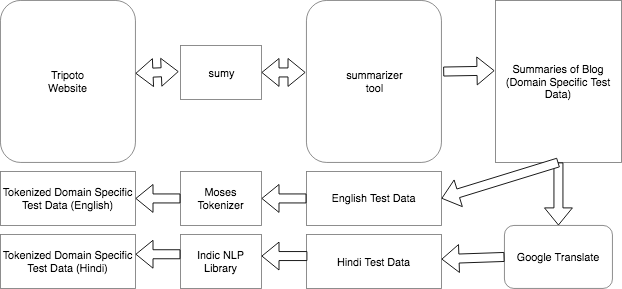
\includegraphics[width=\textwidth]{figures/design4.png}
\caption{Components of the Blog Summarizer Tool.} \label{summarizer}
\end{figure}

The proposed design reflects the structure required to meet the data gathering requirements. The system structure is as follows,

\begin{itemize}
    \item \textbf{Summarizer} The summarizer consists of web-scrapping the blogs from the Tripoto Website and creating summaries of the blogs in five sentences.
    \item \textbf{Text Processing} The Text Processing component consists of creating the Hindi translation using Google Translate and processing the retrived text using different NLP tools.
\end{itemize}

\subsubsection{Summarizer}
The design structure for the processes of Summarizer consists different sub-components, pictured in Figure \ref{summarizer2}

\begin{figure}[h]
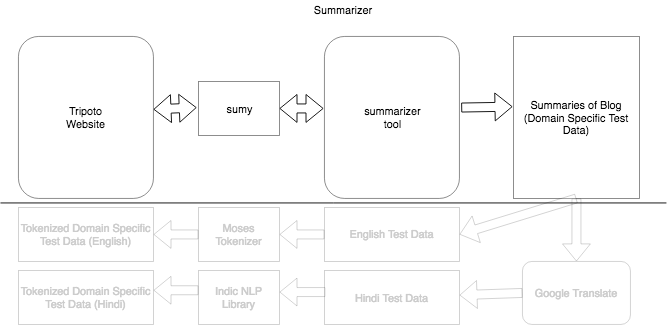
\includegraphics[width=\textwidth]{figures/design5.png}
\caption{Components of the Summarizer.} \label{summarizer2}
\end{figure}

\begin{itemize}
    \item \textbf{Tripoto Website} The Tripoto Website acts as the data source for the Summarizer tool. 
    \item \textbf{sumy} Sumy is an open-source python based library which has implementations for web-scrapping and summarizing. Sumy acts as an interface between the summarizer tool and Tripoto website to generate the Blog summaries.
    \item \textbf{Summarizer Tool} This is the software which generates the domain specific test data. Firstly, it is responsible for generating a list of most popular blogs on Tripoto. Secondly, it must make use of the sumy sub-component to generate the summaries for the blogs.
    \item \textbf{Summaries of Blog} This is the final sub-component of the summarizer which contains the summaries of the Tripoto Blogs.
\end{itemize} 

The Web-scraping and summarizing process involves key design decisions with regard to generation tourism domain sepcific test data. This component must be capable of retrieving the blogs from the Tripoto website and generate summaries simultaneously. 

The components must adhere to the requirements of data quality. Firstly,the tool must be scalable and be able to handle large quantities of data. The tool must have the ability to retrieve any number of blogs from the Tripoto website. Secondly, the tool must avoid duplication of data, and none of the blogs from Tripoto must be repeated for retrieval of data.

\subsubsection{Text Processing}
The design structure for the processes of Text Processing consists of the subset of components, pictured in Figure \ref{summarizer3}.

\begin{figure}[h]
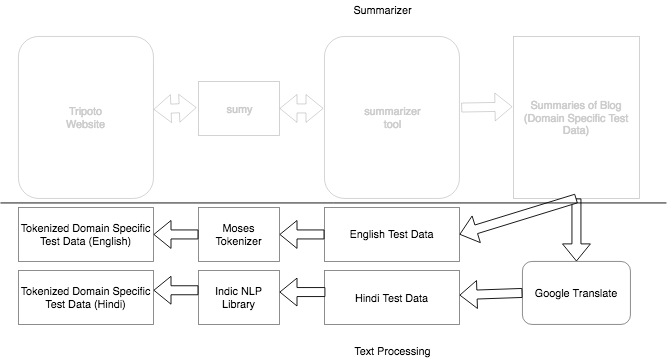
\includegraphics[width=\textwidth]{figures/design6.png}
\caption{Components of the Text Processing.} \label{summarizer3}
\end{figure}

The output from the summarizer tool is saved as the summaries of the blog which becomes the data source for text processing in this component. 

\begin{itemize}
    \item \textbf{Google Translate} The Google Translate acts as the interface between the raw english test data and raw hindi test data. The summaries obtained by the summarizer tool must be translated to hindi raw data using the Google API as it acts as the reference test data for evaluating the quality of translation.
    \item \textbf{English and Hindi Test Data} These sub-components are the data source for the Natural Text Processing phase.
    \item \textbf{Moses Tokenizer} Moses Tokenizer is the interface between the raw english test data and the processed english test data. This system must be able to normalize and tokenize english part of the test data.
    \item \textbf{Indic NLP Library} The Indic NLP library acts as an interface between the raw hindi test data and the processed Hindi test data. This system must be able to normalize and tokenize hindi part of the test ata.
    \item\textbf{Tokenized Domain Specific Test Data} The tokenized domain specific test data in English and Hindi is the output of the system which is an important resource for this research.
\end{itemize}

Core decisions that must be made here involve the methods by which text processing must be done. The text must be normalized and tokenized for further use in the neural machine translation model.This component must ensure that the data quality is met, the data must not be duplicated and the data must be presented in a machine readable form.

\section{Neural Translation Model}

This section discusses the designing of the Neural Translation Model which is used for creating the translations as discussed in the research objectives. 

\subsection{Seq2Seq}
As discussed in the State of Art, the Neural Translation Models is designed using the Seq2Seq model as described by \cite{NIPS2014_5346}. The Figure \ref{seq2seq} shows the basic Sequence to Sequence learning with neural networks. The similar Seq2Seq model with Attention (\cite{DBLP:journals/corr/BahdanauCB14}) is to be designed to meet the research objectives.

\begin{figure}[h]
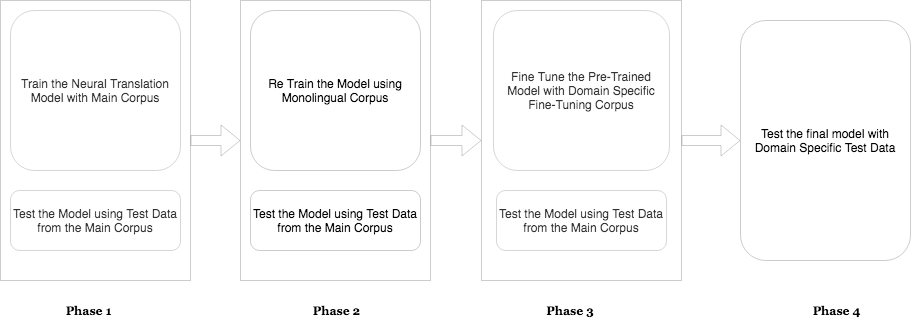
\includegraphics[width=\textwidth]{figures/seq2seq6.png}
\caption{Phases of the Neural Machine Translation Model.} \label{seq2seq}
\end{figure}

\begin{figure}[h]
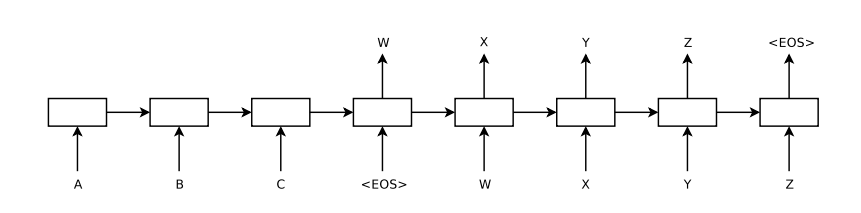
\includegraphics[width=\textwidth]{figures/nmt1.png}
\caption{Sequence to Sequence Learning with Neural Networks. \cite{NIPS2014_5346}} \label{seq2seq}
\end{figure}

\subsection{Training Model}

The training model is to be designed using the Pytorch based implementation of OpenNMT toolkit which provides libraries for designing a neural translation model. The components of the system are captured in Figure \ref{seq2seq1}.

\begin{figure}[h]
\fbox{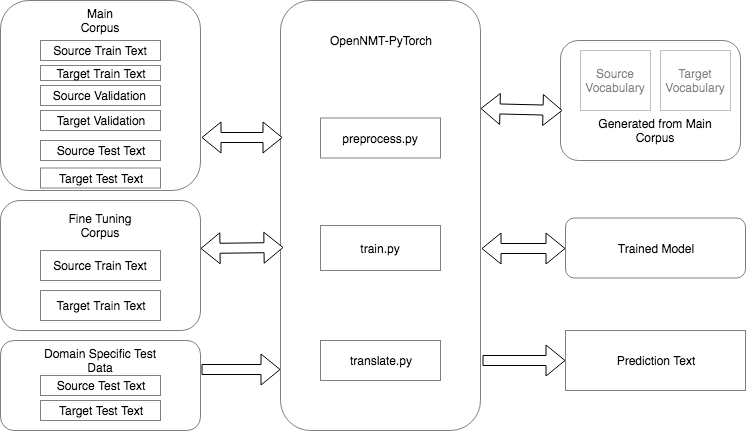
\includegraphics[width=\textwidth]{figures/seq2seq3.png}}
\caption{Components of Neural Translation Model} \label{seq2seq1}
\end{figure}

The proposed design reflects the structure required to meet the research objectives of creating neural translation models. The system structure is as follows,

\begin{itemize}
    \item \textbf{Corpus} The corpus consists of large quantities of parallel bilingual data which is essential for the neural translation model.
    \item \textbf{OpenNMT-PyTorch} The OpenNMT-PyTorch is an open-source PyTorch based toolkit for Neural Machine Translation. This component forms the main unit of the neural translation model which performs all the pre-processing, training and translation tasks.
    \item \textbf{Vocabularies} Vocabularies of Source and Target Languages are generated by the OpenNMT-PyTorch component by utilizing the Corpus. This is further used by the OpenNMT-PyTorch component to train the neural transaltion model.
    \item \textbf{Trained Model} The Trained Model is generated by the OpenNMT-PyTorch compenent by utilising the Corpus and the Vocabularies.
    \item \textbf{Prediction Text} This the output component which is generated by the OpenNMT-PyTorch component by utilizing the corpus and the Trained Model.
\end{itemize}

\subsubsection{Corpus } The first component in the Neural Machine translation system is the Corpus. The Corpus is a  collection of large parallel bilingual data. As discussed in the Data Gathering section, two different corpora and a domain specific test data is used for the neural machine translation task. 
\begin{itemize}
    \item \textbf{Main Corpus} The main corpus is used for initial training of the neural translation model. Firstly, it is used for generating the vocabularies in source and target languages, which is followed by training the model. The main corpus is the IIT-Bombay Hindi-English Parallel Corpus. 
    \item \textbf{Fine Tuning Corpus} The Fine Tuning Corpus is used for the Second-Phase of the training. The pre-trained model from the first phase is used here and it is re-trained using the Fine Tuning Corpus.
    \item \textbf{Domain Specific Test Data} The Domain specific test data is used for generating the domain specific translations and checking the quality of transaltions.
\end{itemize}

\subsubsection{OpenNMT-PyTorch}
\label{sec:opennmt}
OpenNMT is an open source toolkit for neural machine translation and neural sequence modeling. OpenNMT is currently having 3 implementations, OpenNMT-lua which is developed in LuaTorch using Lua programming language, OpenNMT-py which is implemented in PyTorch and OpenNMT-tf which is implemented in TensorFlow. The decision to use the PyTorch implementation of OpenNMT was motivated by the fact that this implementation is easier to extend and well suited for research purposes. This implementation is easy to use as it is Python based and can utilize the GPU power for faster training of the translation models. OpenNMT-PyTorch provides highly configurable models,training procedures and features to improve system performance by a significant margin.

\begin{itemize}
    \item \textbf{preprocess.py} This sub-component pre-processes the training data available in the corpus to generate vocabularies and makes it machine readable for further tasks.
    \item \textbf{train.py} This sub-component trains the translation model by using the Training Data and Validation data from the corpus, and Vocabularies generated by the preprocess.py.
    \item \textbf{translate.py} Translates the Source Test Data from the corpus to the target language.
\end{itemize}

\subsubsection{Vocabularies} 
Vocabularies are generated by the OpenNMT-PyTorch component by processing the training data from the main corpus. These vocabularies are further used by the OpenNMT-PyTorch component to train the main translation model. This component is further used in the second phase, for re-training the model with the domain specific corpus.

The vocabularies must be scalable, as discussed in state of art the vocabularies must be large enough to create good quality translations. 

\subsubsection{Trained Translation Model} 

This sub-component is the translation model trained by the OpenNMT-PyTorch component using the main corpus. This sub-component is used for translating the test data from source text to the target language. 

This sub-component must be capable of translating any text from the source language to the text language and must be able to handle any amount of text data.  

\subsubsection{Prediction Text}

This the output component is generated by the OpenNMT-PyTorch component by utilizing the corpus and the trained model. This text is further used for evaluation of the translation quality.

\subsection{Fine Tuning Pre-trained Model with Domain specific Corpus}
In this section, the design structure for the second phase of the translation task is discussed. The design structure is pictured in Figure \ref{seq2seq2}.

\begin{figure}[h]
\fbox{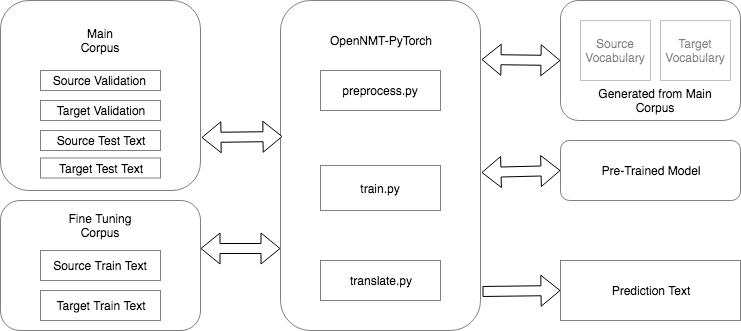
\includegraphics[width=\textwidth]{figures/seq2seq2.png}}
\caption{Fine Tuning of Neural Translation Model} \label{seq2seq2}
\end{figure}


\begin{itemize}
    \item \textbf{Fine-Tuning Corpus} The Fine-Tuning Corpus as discussed in the Data Gathering section is used here to to fine-tune the pre-trained model using the domain specific data. This corpus acts as the new training data for the translation model, where as the validation data and test data remains same as that of the main corpus.
    \item \textbf{Vocabularies generated from Main Corpus} These vocabularies are obtained from the previous phase while pre-processing the training data from the main corpus, and remains unchanged in this phase.
    \item \textbf{Pre-trained Model} The pre-trained Model is the training model that is generated during the first of training with the main corpus. In this phase, the pre-trained model is re-trained using the new training data from fine tuning corpus where as the validation data is used from the main corpus.
    \item \textbf{Predicted Text} The predicted text is the translation text in the target language that is obtained after fine-tuning of the pre-trained model. 
\end{itemize}


\subsection{Testing trained Model with Domain specific test data}
In this section, the design structure for the third phase of the translation task is discussed. The design structure is showed in Figure \ref{seq2seq4}.

\begin{figure}[h]
\fbox{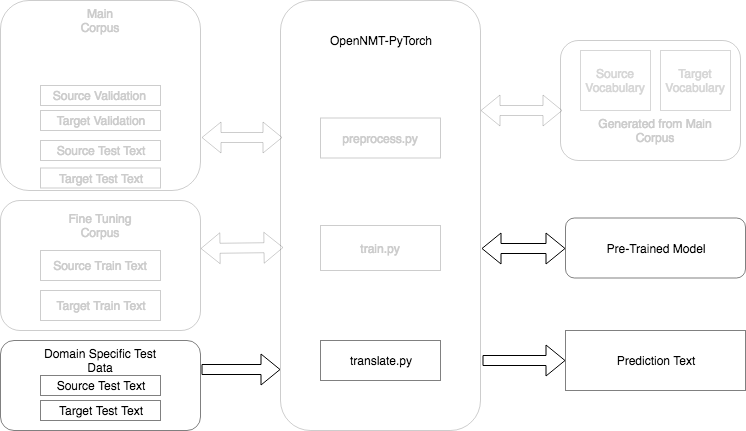
\includegraphics[width=\textwidth]{figures/seq2seq4.png}}
\caption{Components of Neural Translation Model} \label{seq2seq4}
\end{figure}

\begin{itemize}
    \item \textbf{Domain Specific Test Data} As discussed in the data gathering section of this chapter , the domain specific test data is used to test the translation quality in the specific domain. The data is utilized by the translate.py sub-component of the OpenNMT-PyTorch system to generate the translations in the target language.
    \item \textbf{Pre-trained Model} This is the model which is fine-tuned in the second phase, this model is used by the OpenNMT-PyTorch component to translate the domain specific test data into the target language.
    \item \textbf{Prediction Text} The prediction text contains the translation in the target language for the domain specific test data.
\end{itemize}


\section{Visual Interface}
The Visual Interface is intended as a graphic visualization of the predicted data from translation models, allowing for visual display of blog summaries in the Hindi language. See Figure \ref{visualinterface}.

\begin{figure}[h]
\fbox{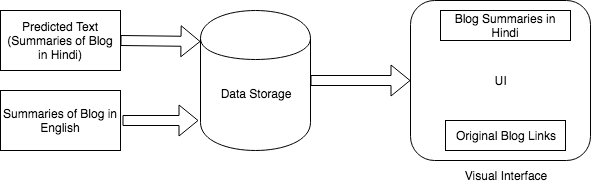
\includegraphics[width=\textwidth]{figures/visualinterface.png}}
\caption{Components of Visual Interface} \label{visualinterface}
\end{figure}

\begin{itemize}
    \item \textbf{Data Storage} Data store for the summaries of blog in English and the predicted text by the neural translation model.
    \item \textbf{User Interface} Displays the summary of the blog in hindi and the original blog link for the selected blog name.
\end{itemize}


The Visual Interface forms an useful platform for demonstrating a resource that could be beneficial to individuals interested in reading blogs in the Hindi language as it is targeted to serve a huge mass of digitally neglected population. The tool will be built as a static web application.

The Visual Interface must be efficient and graphically appealing, as it will display the blogs related to travel. The blog selection option must be capable of displaying the blog summaries in Hindi.

\section{Summary}
In this chapter, a design for the multiple systems allowing the research question to be addressed was proposed. By beginning with a process of data gathering, a set of processes were crafted to achieve the research objectives.The initial section discusses about using a publicly available corpus for training neural translation model, where as the next section discusses methods to generate corpus for fine-tuning the pre-tained model.The following sections gave detail of the components of the systems, and further gave in-depth descriptions of the sub-components of the systems.